% Options for packages loaded elsewhere
\PassOptionsToPackage{unicode}{hyperref}
\PassOptionsToPackage{hyphens}{url}
%
\documentclass[
]{article}
\usepackage{amsmath,amssymb}
\usepackage{lmodern}
\usepackage{ifxetex,ifluatex}
\ifnum 0\ifxetex 1\fi\ifluatex 1\fi=0 % if pdftex
  \usepackage[T1]{fontenc}
  \usepackage[utf8]{inputenc}
  \usepackage{textcomp} % provide euro and other symbols
\else % if luatex or xetex
  \usepackage{unicode-math}
  \defaultfontfeatures{Scale=MatchLowercase}
  \defaultfontfeatures[\rmfamily]{Ligatures=TeX,Scale=1}
\fi
% Use upquote if available, for straight quotes in verbatim environments
\IfFileExists{upquote.sty}{\usepackage{upquote}}{}
\IfFileExists{microtype.sty}{% use microtype if available
  \usepackage[]{microtype}
  \UseMicrotypeSet[protrusion]{basicmath} % disable protrusion for tt fonts
}{}
\makeatletter
\@ifundefined{KOMAClassName}{% if non-KOMA class
  \IfFileExists{parskip.sty}{%
    \usepackage{parskip}
  }{% else
    \setlength{\parindent}{0pt}
    \setlength{\parskip}{6pt plus 2pt minus 1pt}}
}{% if KOMA class
  \KOMAoptions{parskip=half}}
\makeatother
\usepackage{xcolor}
\IfFileExists{xurl.sty}{\usepackage{xurl}}{} % add URL line breaks if available
\IfFileExists{bookmark.sty}{\usepackage{bookmark}}{\usepackage{hyperref}}
\hypersetup{
  pdftitle={Виды анализа и R Markdown},
  pdfauthor={Никитин Никита},
  hidelinks,
  pdfcreator={LaTeX via pandoc}}
\urlstyle{same} % disable monospaced font for URLs
\usepackage[margin=1in]{geometry}
\usepackage{longtable,booktabs,array}
\usepackage{calc} % for calculating minipage widths
% Correct order of tables after \paragraph or \subparagraph
\usepackage{etoolbox}
\makeatletter
\patchcmd\longtable{\par}{\if@noskipsec\mbox{}\fi\par}{}{}
\makeatother
% Allow footnotes in longtable head/foot
\IfFileExists{footnotehyper.sty}{\usepackage{footnotehyper}}{\usepackage{footnote}}
\makesavenoteenv{longtable}
\usepackage{graphicx}
\makeatletter
\def\maxwidth{\ifdim\Gin@nat@width>\linewidth\linewidth\else\Gin@nat@width\fi}
\def\maxheight{\ifdim\Gin@nat@height>\textheight\textheight\else\Gin@nat@height\fi}
\makeatother
% Scale images if necessary, so that they will not overflow the page
% margins by default, and it is still possible to overwrite the defaults
% using explicit options in \includegraphics[width, height, ...]{}
\setkeys{Gin}{width=\maxwidth,height=\maxheight,keepaspectratio}
% Set default figure placement to htbp
\makeatletter
\def\fps@figure{htbp}
\makeatother
\setlength{\emergencystretch}{3em} % prevent overfull lines
\providecommand{\tightlist}{%
  \setlength{\itemsep}{0pt}\setlength{\parskip}{0pt}}
\setcounter{secnumdepth}{-\maxdimen} % remove section numbering
\XeTeXdefaultencoding utf8 \usepackage{xltxtra} \usepackage{fontspec} \setmainfont{Times New Roman} \setsansfont{Arial} \setmonofont{Courier New} \newfontfamily{\cyrillicfont}{Times New Roman} \newfontfamily{\cyrillicfonttt}{Courier New} \newfontfamily{\cyrillicfontsf}{Arial} \usepackage[english,russian]{babel} \XeTeXdefaultencoding cp1251
\ifluatex
  \usepackage{selnolig}  % disable illegal ligatures
\fi

\title{Виды анализа и R Markdown}
\author{Никитин Никита}
\date{25 11 2021}

\begin{document}
\maketitle

\hypertarget{ux440ux430ux437ux432ux435ux434ux43eux447ux43dux44bux439-ux430ux43dux430ux43bux438ux437-ux434ux430ux43dux43dux44bux445}{%
\subsection{Разведочный анализ
данных}\label{ux440ux430ux437ux432ux435ux434ux43eux447ux43dux44bux439-ux430ux43dux430ux43bux438ux437-ux434ux430ux43dux43dux44bux445}}

\hypertarget{ux43fux440ux438ux43cux435ux440}{%
\subsubsection{Пример}\label{ux43fux440ux438ux43cux435ux440}}

Согласно
\href{http://domic.isu.ru/student/entity/5345/content/analysis.pdf}{определению},
цель разведочного анализа данных -- изучить данные и найти взаимосвязи,
о которых ранее не было известно. Разведочный анализ данных:

\begin{itemize}
\tightlist
\item
  Изучает как могут быть связаны различные переменные.
\item
  Полезно для обнаружения новых связей.
\item
  Помогает формулировать гипотезы и управлять планированием будущих
  исследований и сбора данных.
\end{itemize}

\href{https://ru.wikipedia.org/wiki/\%D0\%A0\%D0\%B0\%D0\%B7\%D0\%B2\%D0\%B5\%D0\%B4\%D0\%BE\%D1\%87\%D0\%BD\%D1\%8B\%D0\%B9_\%D0\%B0\%D0\%BD\%D0\%B0\%D0\%BB\%D0\%B8\%D0\%B7_\%D0\%B4\%D0\%B0\%D0\%BD\%D0\%BD\%D1\%8B\%D1\%85}{Также}
одной из целей разведочного анализа данных является \textbf{обнаружение
отклонений и аномалий} в данных.

Рассмотрим пример
{[}исследования{]}(\url{https://cyberleninka.ru/article/n/bezrabotitsa-kak-odna-iz-globalnyh-problem-sovremennogo-mira},
В статье проведен анализ уровня безработицы за 2015-2017 гг., найдены
различные связи различных переменных, обозреваются различные причины
безработицы:

\begin{quote}
--- Уровень безработицы -- экономический показатель, один из основных
индикаторов на рынке труда. Он отражает соотношение между
нетрудоустроенными гражданами в обществе и теми, кто имеет постоянную
работу.
\end{quote}

Иными словами, требовалось выявить возможные зависимости безработицы в
мире от определённых факторов.

В статье используются данные Росстата, Евростата и ОЭСР, проблема
безработицы анализируется на международном уровне.

Безработица, незащищенная занятость и работающие бедные -- тенденции и
прогнозы на 2016-18 гг.:

\begin{longtable}[]{@{}llll@{}}
\toprule
млн. чел / год & 2016 & 2017 & 2018 \\
\midrule
\endhead
В мире & 197,7 & 201,1 & 203,8 \\
Развитые страны & 38,6 & 37,9 & 38 \\
Страны с формирующимся рынком & 143,4 & 147 & 149 \\
Развивающиеся страны & 15,7 & 16,1 & 16,6 \\
\bottomrule
\end{longtable}

В рамках исследования была построена линейный график уровня безработицы:
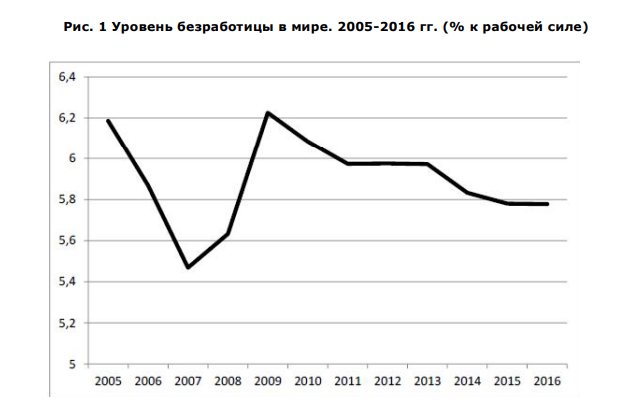
\includegraphics{C:/Users/nicki/Downloads/markdown/Capture1.PNG}

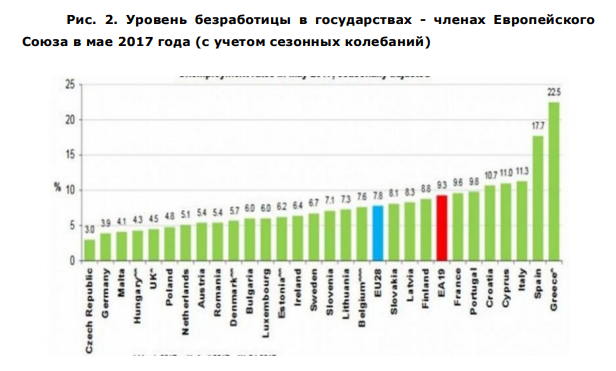
\includegraphics{C:/Users/nicki/Downloads/markdown/Capture.PNG}

В ходе исследования рассматривались страны:

\begin{enumerate}
\def\labelenumi{\arabic{enumi}.}
\tightlist
\item
  Англия;
\item
  Германия;
\item
  Швецария;
\item
  Ирландия;
\item
  Испания;
\item
  Греция;
\end{enumerate}

\hypertarget{ux432ux44bux432ux43eux434ux44b}{%
\subsubsection{Выводы}\label{ux432ux44bux432ux43eux434ux44b}}

Исследование использует методы \textbf{разведочного анализа данных},
чтобы обнаружить \textbf{взаимосвязи между переменными, о которых
заранее неизвестно} (например, взаимосвязь между переменной,
характеризующей год, и переменной, характеризующей процент безработицы).

\hypertarget{ux43cux435ux445ux430ux43dux438ux441ux442ux438ux447ux435ux441ux43aux438ux439-ux430ux43dux430ux43bux438ux437-ux434ux430ux43dux43dux44bux445}{%
\subsection{Механистический анализ
данных}\label{ux43cux435ux445ux430ux43dux438ux441ux442ux438ux447ux435ux441ux43aux438ux439-ux430ux43dux430ux43bux438ux437-ux434ux430ux43dux43dux44bux445}}

\hypertarget{ux43fux440ux438ux43cux435ux440-1}{%
\subsubsection{Пример}\label{ux43fux440ux438ux43cux435ux440-1}}

Согласно
\href{http://domic.isu.ru/student/entity/5345/content/analysis.pdf}{определению},
цель механистического анализа данных -- понять, какие именно изменения в
переменных приводят к точным изменениям в других переменных.
Механистический анализ данных применяется для:

\begin{itemize}
\tightlist
\item
  Применяется к простым ситуациям или ситуациям, которые хорошо
  моделируются детерминированными уравнениями.
\item
  Обычно применяется к физическим или инженерным наукам.
\item
  Например: биологические науки слишком «шумны» для использования
  механистического анализа.
\item
  Часто единственный шум в данных -- ошибки измерения.
\end{itemize}

Рассмотрим пример
\href{https://cyberleninka.ru/article/n/chislennaya-model-rascheta-radiotrass-korotkih-radiovoln-v-ionosfere}{исследования},
целью которого являлся проведение расчетов радиотрасс в авроральной
ионосфере и поглощения радиоволн вдоль них в зависимости от выбора
геофизических условий.

Использовано уравнение баланса процессов ионизации и рекомбинации в
ионосфере:

\[{\Delta N = -N + \sqrt{N^2+q/a}}\]

где α --- коэффициент рекомбинации; Ne0 --- фоновая концентрация
электронов по модели IRI; ∆q --- функция корпускулярной ионизации
молекул нейтральной атмосферы авроральными электронами, высыпающимися из
магнитосферы в ионосферу; q0 --- фоновое значение функции ионизации.

Некоторые из результатов расчетов получены для зимних условий 22.12.1969
г. при среднем уровне солнечной и геомагнитной активности (F10,7 = 150,
Ap = 27). Для этих условий обнаружено более слабое развитие дневного
слоя \(F2\) ионосферы по модели IRI по сравнению с результатами
модельных расчетов и данными экспериментальных ионо- грамм для
радиотрассы Мурманск --- Санкт-Петербург . На основе данных по
параметрам \(NmF2\) и \(hmF2\) из {[}9{]} проведена дополнительная
коррекция высотных профилей \(Ne(h)\) электронной концентрации модели .
На рисунке слева показан пример профиля Ne(h) модели IRI над станцией
(65°N, 290°E) в указанных условиях для мирового времени 16,6 ч, а справа
--- его коррекция

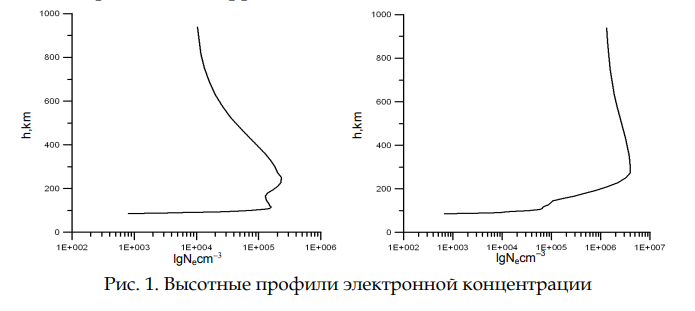
\includegraphics{C:/Users/nicki/Downloads/markdown/Capture3.PNG}

\hypertarget{ux432ux44bux432ux43eux434ux44b-1}{%
\subsubsection{Выводы}\label{ux432ux44bux432ux43eux434ux44b-1}}

Поскольку рассмотренное исследование имело дело с ситуацией, которая
может быть смоделирована с помощью уравнения, а также обнаружило
определённую связь между переменными с высоким уровнем доверия, можно
считать, что исследование использовано механистический анализ данных.

\end{document}
